\appendix

\section{Implementation Details}
\label{appendix:impl}

\paragraph{Models and decoding.}
We use the public checkpoints of Qwen2.5-Omni-7B (28 decoder layers), MiniCPM-o~4.5 (36 decoder layers), and Qwen3-Omni-30B-A3B-Instruct (48 decoder layers) in half precision (bfloat16) on two B200 GPUs, with greedy decoding, no repetition penalty, and at most 512 new tokens.
The late band of \Cref{sec:scoring} is the last third of the layers: 18--27, 24--35, and 32--47.

\paragraph{Inputs and units.}
\emph{Video.} Qwen2.5-Omni samples two frames per second within a budget of about 20k video tokens; its encoder groups two frames into one temporal step of about 1.02\,s, which is our unit. MiniCPM-o~4.5 samples one frame per second with 64 tokens per frame, and each frame is a unit. Unit times are taken from the encoder's own time grid. Videos are between 10 and 90\,s long and are given without the audio track.
\emph{Audio.} Clips are cut into one-second units along the audio encoder's token sequence.
\emph{Image--text.} Each of the 15 quotes is a unit. Quotes are given in the order of MMDocRAG, text passages first and images after them, followed by the question. Images use each model's standard image processing.
Positions outside the units (system prompt, template tokens, question, options, instruction, and whitespace) are never candidates.

\paragraph{Prompts.}
For multiple-choice questions the instruction is: ``\emph{Answer the question based on the \{video, audio\} provided. Explain your reasoning step by step. End your response with a final line of the form "Answer: X", where X is the option letter.}''
MMAU puts the correct answer first in almost half of its questions, so we shuffle the options with a fixed seed.
For the self-citation baseline the instruction adds: ``\emph{After each sentence that uses information from the \{video, audio\}, cite the time span it comes from in seconds, e.g.\ [12.0-15.5s].}'' For documents it asks for quote ids in MMDocRAG's citation format.

\paragraph{Sentences.}
Responses are split into sentences with spaCy and at line breaks. Sentences are aligned to the generated token ids, so each generated token belongs to one sentence.

\paragraph{OmniTrace-trained.}
\label{appendix:trained}
The trained variant of \Cref{sec:scoring} keeps every part of OmniTrace and changes only the head weights. The feature of a head is the attention mass it places on a unit, summed over the generated tokens of the sentence or the response, for every head of the decoder ($28\times28$ in Qwen2.5-Omni-7B), recorded in one replay of the response. With equal weights on the last third of the layers and zero elsewhere the score is the default of \Cref{eq:mass}, and training starts from these weights.
The training signal is 32 random ablations per question, in which each unit is hidden with probability 0.5 by the placeholders of \Cref{sec:protocol}. The loss is one minus the Pearson correlation between the predicted and the measured log-probability over the ablations, for responses and their sentences, minimized with Adam and early stopping on 15\% of the training questions. This objective follows AT2~\cite{cohenwang2025at2}, which is defined for text sources and has no released weights for omni-modal models; the features, the units, the ablations, and all weights here are ours.
We cross-fit in five folds, so each question is scored with weights trained on the other four.
Training costs 32 ablation passes for every training question, once per model; nothing is added at test time.
On held-out questions of Qwen2.5-Omni the trained score predicts the ablation outcomes about as well as the default on video (correlation 0.33 against 0.34) and better on audio (0.61 against 0.58) and image--text input (0.85 against 0.78). About a third of the absolute weight stays on the late layers, and about half of the weights are negative.
For labels we clip negative scores at zero and apply \Cref{eq:label} unchanged. These labels agree with human evidence better than the default's (F1 of 0.30 against 0.20 on video and 0.50 against 0.48 on documents for Qwen2.5-Omni; 0.30 against 0.14 and 0.56 against 0.26 for MiniCPM-o~4.5); we did not test them causally.

\paragraph{Reading attention.}
We run the model with its standard scaled-dot-product attention and recompute, in the late layers only, the attention row of the last position at each step. Against the attention maps returned by the framework, the largest absolute difference is $2\times10^{-7}$, and the generated tokens are identical.

\paragraph{Development study.}
The observations in \Cref{sec:design} come from 1{,}000 NExT-GQA questions on 637 videos. The 300 test questions are drawn from other videos.
Agreement with human spans was measured on the answer sentences of the 655 correctly answered questions.
We then compared the candidate settings with the causal test on 200 of these questions and fixed the setting of \Cref{eq:mass} before running any test question, any audio or image--text question, and the second model.

\section{Details of the Causal Test}
\label{appendix:causal}

\paragraph{Placeholders.}
A hidden video unit is replaced by black frames, an audio unit by silence at the clip's noise floor, an image by a black image of the same size, and a text passage by blank tokens of the same count. We verified on video that only the tokens of the hidden unit change.

\paragraph{Budgets and controls.}
For a budget $b$ on audio and video we hide the top-ranked units up to a share $b$ of the duration; for documents we hide the top $k$ quotes. Random controls hide the same number of units, with three draws per question. Keep tests hide all candidate units except the selected ones, with the same controls.
For the sentence-level test we take the top units by the sentence's own scores.
Intervals are 95\% percentile intervals from 1{,}000 bootstrap resamples of the questions (of the sentences for sentence-level metrics).

\paragraph{Two evaluation runs.}
The baselines were evaluated in a second run that tests OmniTrace again next to them. The drop for OmniTrace's top units is identical in the two runs; the random draws differ. This is why the lift of OmniTrace differs slightly between \Cref{tab:baselines} and \Cref{tab:models} (for example 0.077 and 0.069 on audio). Each paired comparison uses rows from one run.

\paragraph{Coverage.}
A few questions ran out of GPU memory in the replay and are left out: on MiniCPM-o~4.5, 13 of 246 video and 9 of 196 audio questions; on Qwen2.5-Omni, 2 video questions in the label test and 16 in the self-citation test.

\subsection{Masking Choice}
\label{appendix:masking}

\begin{table*}[t]
\centering
\small
% generated by analysis/paper_models.py; do not edit by hand
\begin{tabular}{llcccc}
\toprule
\textbf{Model} & \textbf{Modality} ($n$) & Budget & Lift, empty & Lift, mean & Mean $-$ empty (paired) \\
\midrule
Qwen2.5-Omni-7B & Video (246) & 10\% & 0.007 & 0.007 & 0.000 {\tiny[$-$0.002, 0.003]} \\
 &  & 20\% & 0.016 & 0.014 & $-$0.002 {\tiny[$-$0.004, 0.000]} \\
 &  & 30\% & 0.017 & 0.017 & 0.000 {\tiny[$-$0.001, 0.001]} \\
 &  & 50\% & 0.027 & 0.025 & $-$0.002 {\tiny[$-$0.008, 0.003]} \\
 & Audio (196) & 10\% & 0.056 & 0.062 & 0.006 {\tiny[$-$0.002, 0.013]} \\
 &  & 20\% & 0.069 & 0.078 & 0.009 {\tiny[0.000, 0.018]} \\
 &  & 30\% & 0.068 & 0.076 & 0.008 {\tiny[0.001, 0.016]} \\
 &  & 50\% & 0.060 & 0.072 & 0.012 {\tiny[$-$0.010, 0.033]} \\
\midrule
MiniCPM-o 4.5 & Video (233) & 10\% & 0.006 & 0.007 & 0.002 {\tiny[$-$0.001, 0.004]} \\
 &  & 20\% & 0.027 & 0.028 & 0.001 {\tiny[$-$0.001, 0.004]} \\
 &  & 30\% & 0.050 & 0.054 & 0.004 {\tiny[0.001, 0.007]} \\
 &  & 50\% & 0.073 & 0.076 & 0.003 {\tiny[$-$0.001, 0.007]} \\
 & Audio (187) & 10\% & 0.102 & 0.098 & $-$0.004 {\tiny[$-$0.020, 0.011]} \\
 &  & 20\% & 0.143 & 0.138 & $-$0.005 {\tiny[$-$0.018, 0.009]} \\
 &  & 30\% & 0.135 & 0.136 & 0.001 {\tiny[$-$0.014, 0.016]} \\
 &  & 50\% & 0.097 & 0.110 & 0.014 {\tiny[0.003, 0.025]} \\
\bottomrule
\end{tabular}

\caption{Lift of OmniTrace under two ways of hiding a unit, on the same questions: a content-free placeholder at the input (\emph{empty}, used throughout the paper) and replacing the unit's embeddings by their mean (\emph{mean}).}
\label{tab:masking}
\end{table*}

\Cref{tab:masking} repeats the response-level test with the mean-embedding replacement.
On video and audio the lifts under the two fills are close for both models, most paired differences include zero, and the others are small.
We do not use the mean replacement for image--text input. A text passage whose tokens are all replaced by the same mean embedding is far from anything the model has seen: hiding one random passage this way costs 1.70 nats per token regardless of the passage, against 0.03 with blank tokens. Such a test measures the damage of the replacement, not the role of the passage.

\subsection{Replay Agreement}
\label{appendix:replay}

With greedy decoding, the token with the highest probability in the replay should be the generated token.
For MiniCPM-o~4.5 this holds at 97--98\% of the positions. For Qwen2.5-Omni-7B it holds at 88\% (video), 86\% (audio), and 81\% (image--text).
The gap comes from the generation path in half precision: on a sample of audio questions, a response generated in single precision is replayed with full agreement, and replaying a half-precision response gives the same values in half and in single precision, so the replay itself is accurate.
All drops in the paper compare two replays of the same tokens, with and without hidden units, so they are internally consistent.

\section{Baselines}
\label{appendix:baselines}

All baselines write one score per unit for the response and for each sentence, and are then evaluated by the same code as OmniTrace.

\paragraph{Embedding similarity.}
A unit is scored by the cosine similarity between the sentence and the unit. Video frames and images are embedded with SigLIP (\texttt{siglip-so400m-patch14-384}), one-second audio slices with CLAP (\texttt{clap-htsat-unfused}), and text passages with a text encoder (\texttt{bge-base-en-v1.5}). A video unit is the mean over its frames. Image and text similarities are on different scales, so for documents they are standardized within each modality. The response-level score is the mean over sentences.

\paragraph{Self-citation.}
The model is run again with the citation prompt of \Cref{appendix:impl}. A cited time span selects the units it overlaps, and a cited quote id selects that quote. Because the responses of this run differ from the main run, we compare the cited units with OmniTrace's top units of the same count on the responses of the citation run. Responses without a valid citation have no cited set and are not scored.

\paragraph{Leave-one-out.}
Each unit is hidden alone, and its score is the drop in the mean log-probability of the response or the sentence. The cost is one forward pass per unit (41, 17, and 16 on average for video, audio, and image--text).

\paragraph{ContextCite.}
We draw 32 random ablations in which each unit is kept with probability 0.5, and fit a Lasso model (regularization 0.01) that predicts the log-probability of the response or sentence from the kept units; its weights are the scores.

Both perturbation baselines use the placeholders and the teacher-forced target of the causal test itself.

\paragraph{Modalities.}
Leave-one-out is a generic procedure and ContextCite is defined for text contexts, where a source is removed by deleting its tokens. Neither has a published form for audio, video, or mixed image--text input. In this paper both run on the source units of OmniTrace and remove a unit with the content-free placeholders of \Cref{sec:protocol}; their numbers on audio, video, and images exist only through this extension.

\section{Additional Results}
\label{appendix:additional}

\subsection{Baselines on MiniCPM-o 4.5}
\label{appendix:minicpm}

\begin{table*}[t]
\centering
\small
\setlength{\tabcolsep}{4.2pt}
\resizebox{\textwidth}{!}{% generated by analysis/paper_models.py; do not edit by hand
\begin{tabular}{lrcccrcccrccc}
\toprule
 & \multicolumn{4}{c}{\textbf{Video} ($n$ = 246)} & \multicolumn{4}{c}{\textbf{Audio} ($n$ = 196)} & \multicolumn{4}{c}{\textbf{Image--text} ($n$ = 400)} \\
\cmidrule(lr){2-5}\cmidrule(lr){6-9}\cmidrule(lr){10-13}
\textbf{Method} & Fwd & Lift & S-lift & S-spec & Fwd & Lift & S-lift & S-spec & Fwd & Lift & S-lift & S-spec \\
\midrule
\multicolumn{13}{>{\columncolor{gray!15}}l}{\textit{Baselines on MiniCPM-o 4.5}}\\
Embedding similarity & 0 & 0.030 & 0.032 & 0.013 & 0 & 0.067\mdn & 0.055\mdn & 0.015\mdn & 0 & 0.248\mup & 0.365\mup & 0.282\mup \\
Self-citation$^\dagger$ & 1$^\ddagger$ & 0.026\mup & 0.037\mup & \textbf{0.034}\mup & 1$^\ddagger$ & 0.064\mdn & 0.093\mdn & \textbf{0.114}\mdn & 1$^\ddagger$ & 0.267\mup & \textbf{0.907}\mup & \textbf{0.903}\mup \\
Leave-one-out$^\ast$ & 41 & 0.037\mup & 0.039\mup & 0.027\mup & 17 & \underline{0.189}\mup & \underline{0.152}\mup & 0.086\mup & 16 & \underline{0.451}\mup & \underline{0.736}\mup & \underline{0.545}\mup \\
ContextCite$^\ast$ & 33 & \underline{0.050}\mup & \underline{0.058}\mup & \underline{0.032}\mup & 28 & \textbf{0.193}\mup & \textbf{0.157}\mup & \underline{0.101}\mup & 33 & \textbf{0.453}\mup & 0.722\mup & 0.542\mup \\
\midrule
\multicolumn{13}{>{\columncolor{gray!15}}l}{\textit{OmniTrace on MiniCPM-o 4.5}}\\
\textbf{OmniTrace} (ours) & 0 & 0.024 & 0.027 & 0.012 & 0 & 0.136 & 0.102 & 0.047 & 0 & 0.105 & 0.159 & 0.098 \\
\textbf{OmniTrace-trained} (ours)$^\P$ & 0 & \textbf{0.067}\mup & \textbf{0.065}\mup & 0.024\mup & 0 & 0.169\mup & 0.120\mup & 0.054 & 0 & 0.432\mup & 0.706\mup & 0.507\mup \\
\bottomrule
\end{tabular}
}
\caption{The comparison of \Cref{tab:baselines} repeated on MiniCPM-o~4.5: every baseline and both OmniTrace variants are run on this model. Columns and marks as in \Cref{tab:baselines}; arrows compare with OmniTrace on this model. Self-citation is scored on the 210, 92, and 227 responses that cite; the document citation run covers 252 of the 400 questions.}
\label{tab:baselines_minicpm}
\end{table*}

\Cref{tab:baselines_minicpm} repeats the baseline comparison on the second model, with the setting of OmniTrace unchanged.

\emph{Audio.} OmniTrace has 1.4 to 2 times the lift of embedding similarity at every budget, and reaches 52\%, 72\%, 75\%, and 95\% of leave-one-out's lift at the four budgets and 62--92\% of OmniTrace-trained's.
Where the model cites, OmniTrace's units of the same count matter 1.5 times as much as the cited spans at response level and twice as much at sentence level.

\emph{Video.} The result depends on the budget. As a share of leave-one-out's lift OmniTrace reaches 27\%, 65\%, 147\%, and 194\% at the four budgets, and from 30\% on it is level with ContextCite. Its keep gain is reliably above that of embedding similarity from 20\% on. OmniTrace-trained is ahead of every method at every budget.

\emph{Image--text.} OmniTrace reaches 23\% of the lift of leave-one-out and ContextCite at two quotes (39\% at three) and 42\% of embedding similarity. This is the setting in which the fixed reading transfers worst.

\emph{What training finds.} OmniTrace-trained reads the same attention with fitted head weights. It stays within 11\% of leave-one-out on audio and documents and is the best method on video, at no test-time cost. On held-out questions its score predicts the ablation outcomes far better than the fixed setting (correlation 0.45, 0.58, and 0.94 against 0.23, 0.24, and 0.52 for video, audio, and documents), and only 18--21\% of its absolute weight lies on the late layers, against 35\% on Qwen2.5-Omni.
The evidence is therefore present in the attention of this model, in other layers than the ones the fixed setting sums. A rule that selects layers or heads without perturbation data would remove this gap; we leave it open.

\emph{Citations.} MiniCPM-o~4.5 cites in 85\%, 51\%, and 90\% of its video, audio, and document responses. Its cited video seconds and quotes have a larger lift than OmniTrace's units of the same count, and its cited audio spans a smaller one. With the citation prompt its accuracy changes from 77.0\% to 75.7\% on video and from 76.3\% to 70.7\% on audio.

\subsection{All Budgets}
\label{appendix:budgets}

\begin{figure}[t]
\centering
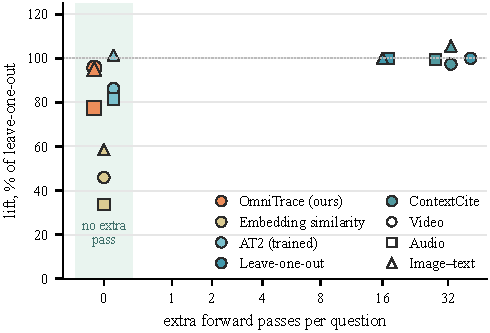
\includegraphics[width=\columnwidth]{media/figure/fig_cost.pdf}
\caption{\textbf{Faithfulness against cost} on Qwen2.5-Omni-7B (the panel of \Cref{fig:teaser}). Lift of each method as a share of leave-one-out's lift, against the extra forward passes it needs per question. Both OmniTrace variants sit in the shaded column: they read their scores from the generation pass. OmniTrace-trained needs ablation data from the same model beforehand.}
\label{fig:cost}
\end{figure}

\begin{table*}[t]
\centering
\small
\resizebox{\textwidth}{!}{% generated by analysis/paper_models.py; do not edit by hand
\begin{tabular}{llcccccc}
\toprule
\textbf{Model} & \textbf{Modality} ($n$) & Budget & Drop, top & Drop, random & Lift & Lift $>0$ & Keep gain \\
\midrule
Qwen2.5-Omni-7B & Video (246) & 10\% & 0.009 & 0.002 & 0.007 {\tiny[0.005, 0.009]} & 70\% & 0.022 {\tiny[0.006, 0.048]} \\
 &  & 20\% & 0.020 & 0.004 & 0.016 {\tiny[0.011, 0.021]} & 73\% & 0.010 {\tiny[$-$0.002, 0.021]} \\
 &  & 30\% & 0.025 & 0.009 & 0.017 {\tiny[0.013, 0.021]} & 77\% & 0.006 {\tiny[$-$0.004, 0.013]} \\
 &  & 50\% & 0.043 & 0.016 & 0.027 {\tiny[0.021, 0.034]} & 88\% & 0.005 {\tiny[$-$0.000, 0.011]} \\
 & Audio (196) & 10\% & 0.112 & 0.056 & 0.056 {\tiny[0.043, 0.069]} & 72\% & 0.042 {\tiny[0.033, 0.053]} \\
 &  & 20\% & 0.144 & 0.075 & 0.069 {\tiny[0.055, 0.086]} & 75\% & 0.066 {\tiny[0.051, 0.080]} \\
 &  & 30\% & 0.167 & 0.099 & 0.068 {\tiny[0.054, 0.083]} & 77\% & 0.073 {\tiny[0.058, 0.090]} \\
 &  & 50\% & 0.208 & 0.149 & 0.060 {\tiny[0.046, 0.073]} & 73\% & 0.080 {\tiny[0.063, 0.098]} \\
 & Image--text (400) & 1 quote & 0.314 & 0.031 & 0.282 {\tiny[0.250, 0.319]} & 92\% & 0.356 {\tiny[0.309, 0.407]} \\
 &  & 2 quotes & 0.423 & 0.076 & 0.348 {\tiny[0.310, 0.383]} & 95\% & 0.412 {\tiny[0.371, 0.456]} \\
 &  & 3 quotes & 0.485 & 0.109 & 0.377 {\tiny[0.338, 0.418]} & 94\% & 0.396 {\tiny[0.358, 0.438]} \\
\midrule
MiniCPM-o 4.5 & Video (233) & 10\% & 0.019 & 0.013 & 0.006 {\tiny[0.002, 0.010]} & 55\% & 0.010 {\tiny[$-$0.000, 0.020]} \\
 &  & 20\% & 0.046 & 0.019 & 0.027 {\tiny[0.019, 0.034]} & 73\% & 0.026 {\tiny[0.018, 0.034]} \\
 &  & 30\% & 0.078 & 0.028 & 0.050 {\tiny[0.039, 0.062]} & 79\% & 0.031 {\tiny[0.024, 0.039]} \\
 &  & 50\% & 0.123 & 0.050 & 0.073 {\tiny[0.060, 0.087]} & 85\% & 0.021 {\tiny[0.016, 0.026]} \\
 & Audio (187) & 10\% & 0.204 & 0.102 & 0.102 {\tiny[0.077, 0.131]} & 63\% & 0.060 {\tiny[0.039, 0.081]} \\
 &  & 20\% & 0.272 & 0.129 & 0.143 {\tiny[0.113, 0.174]} & 72\% & 0.106 {\tiny[0.079, 0.133]} \\
 &  & 30\% & 0.307 & 0.172 & 0.135 {\tiny[0.107, 0.162]} & 68\% & 0.128 {\tiny[0.101, 0.158]} \\
 &  & 50\% & 0.370 & 0.273 & 0.097 {\tiny[0.074, 0.121]} & 65\% & 0.125 {\tiny[0.098, 0.151]} \\
 & Image--text (400) & 1 quote & 0.145 & 0.078 & 0.067 {\tiny[0.048, 0.089]} & 58\% & 0.039 {\tiny[0.023, 0.057]} \\
 &  & 2 quotes & 0.269 & 0.164 & 0.105 {\tiny[0.076, 0.130]} & 64\% & 0.074 {\tiny[0.052, 0.096]} \\
 &  & 3 quotes & 0.414 & 0.221 & 0.194 {\tiny[0.167, 0.222]} & 75\% & 0.154 {\tiny[0.131, 0.178]} \\
\midrule
Qwen3-Omni-30B-A3B & Video (246) & 10\% & 0.022 & 0.003 & 0.019 {\tiny[0.014, 0.024]} & 70\% & 0.019 {\tiny[0.012, 0.027]} \\
 &  & 20\% & 0.038 & 0.005 & 0.033 {\tiny[0.025, 0.040]} & 74\% & 0.016 {\tiny[0.011, 0.021]} \\
 &  & 30\% & 0.047 & 0.008 & 0.038 {\tiny[0.030, 0.047]} & 76\% & 0.010 {\tiny[0.006, 0.015]} \\
 &  & 50\% & 0.061 & 0.015 & 0.046 {\tiny[0.037, 0.055]} & 77\% & 0.006 {\tiny[0.004, 0.009]} \\
 & Audio (196) & 10\% & 0.142 & 0.060 & 0.083 {\tiny[0.065, 0.103]} & 75\% & 0.059 {\tiny[0.044, 0.075]} \\
 &  & 20\% & 0.191 & 0.079 & 0.112 {\tiny[0.088, 0.137]} & 78\% & 0.097 {\tiny[0.074, 0.118]} \\
 &  & 30\% & 0.215 & 0.116 & 0.099 {\tiny[0.078, 0.125]} & 76\% & 0.100 {\tiny[0.078, 0.126]} \\
 &  & 50\% & 0.262 & 0.180 & 0.082 {\tiny[0.065, 0.100]} & 75\% & 0.094 {\tiny[0.076, 0.114]} \\
 & Image--text (400) & 1 quote & 0.276 & 0.044 & 0.232 {\tiny[0.213, 0.252]} & 96\% & 0.209 {\tiny[0.188, 0.229]} \\
 &  & 2 quotes & 0.415 & 0.099 & 0.316 {\tiny[0.294, 0.338]} & 98\% & 0.304 {\tiny[0.284, 0.329]} \\
 &  & 3 quotes & 0.495 & 0.131 & 0.363 {\tiny[0.342, 0.386]} & 99\% & 0.355 {\tiny[0.332, 0.379]} \\
\bottomrule
\end{tabular}
}
\caption{Response-level results of OmniTrace at every budget. Drops are in nats per token. Lift $>0$: share of the questions with a positive lift. Brackets: 95\% bootstrap intervals.}
\label{tab:budget}
\end{table*}

\begin{table*}[t]
\centering
\small
\setlength{\tabcolsep}{4pt}
\resizebox{\textwidth}{!}{% generated by analysis/paper_models.py; do not edit by hand
\begin{tabular}{llccccccc}
\toprule
 & & & \multicolumn{3}{c}{Lift} & \multicolumn{3}{c}{OmniTrace $-$ baseline (paired)} \\
\cmidrule(lr){4-6}\cmidrule(lr){7-9}
\textbf{Modality} & Budget & OmniTrace & Embedding & Leave-one-out & ContextCite & Embedding & Leave-one-out & ContextCite \\
\midrule
Video & 10\% & 0.007 & 0.002 & 0.014 & 0.013 & 0.005 {\tiny[0.002, 0.009]} & $-$0.007 {\tiny[$-$0.011, $-$0.005]} & $-$0.006 {\tiny[$-$0.008, $-$0.003]} \\
 & 20\% & 0.016 & 0.008 & 0.016 & 0.016 & 0.008 {\tiny[0.004, 0.013]} & $-$0.001 {\tiny[$-$0.004, 0.003]} & $-$0.000 {\tiny[$-$0.005, 0.006]} \\
 & 30\% & 0.020 & 0.012 & 0.019 & 0.022 & 0.008 {\tiny[0.004, 0.013]} & 0.001 {\tiny[$-$0.003, 0.006]} & $-$0.002 {\tiny[$-$0.006, 0.002]} \\
 & 50\% & 0.027 & 0.019 & 0.020 & 0.031 & 0.008 {\tiny[0.002, 0.014]} & 0.007 {\tiny[0.003, 0.011]} & $-$0.004 {\tiny[$-$0.009, 0.001]} \\
\midrule
Audio & 10\% & 0.060 & 0.023 & 0.090 & 0.087 & 0.037 {\tiny[0.024, 0.049]} & $-$0.030 {\tiny[$-$0.038, $-$0.023]} & $-$0.027 {\tiny[$-$0.035, $-$0.019]} \\
 & 20\% & 0.077 & 0.034 & 0.100 & 0.099 & 0.044 {\tiny[0.031, 0.057]} & $-$0.022 {\tiny[$-$0.030, $-$0.014]} & $-$0.022 {\tiny[$-$0.030, $-$0.015]} \\
 & 30\% & 0.074 & 0.037 & 0.092 & 0.096 & 0.037 {\tiny[0.025, 0.049]} & $-$0.017 {\tiny[$-$0.024, $-$0.011]} & $-$0.021 {\tiny[$-$0.028, $-$0.015]} \\
 & 50\% & 0.057 & 0.041 & 0.064 & 0.071 & 0.016 {\tiny[0.008, 0.024]} & $-$0.006 {\tiny[$-$0.011, $-$0.002]} & $-$0.014 {\tiny[$-$0.018, $-$0.009]} \\
\midrule
Image--text & 1 quote & 0.285 & 0.142 & 0.317 & 0.311 & 0.143 {\tiny[0.115, 0.172]} & $-$0.032 {\tiny[$-$0.041, $-$0.024]} & $-$0.026 {\tiny[$-$0.034, $-$0.018]} \\
 & 2 quotes & 0.351 & 0.216 & 0.368 & 0.389 & 0.135 {\tiny[0.107, 0.166]} & $-$0.018 {\tiny[$-$0.033, 0.000]} & $-$0.039 {\tiny[$-$0.054, $-$0.022]} \\
 & 3 quotes & 0.379 & 0.257 & 0.380 & 0.431 & 0.122 {\tiny[0.098, 0.148]} & $-$0.002 {\tiny[$-$0.023, 0.025]} & $-$0.052 {\tiny[$-$0.074, $-$0.033]} \\
\bottomrule
\end{tabular}
}
\caption{Lift of every method at every budget on Qwen2.5-Omni-7B, and the paired difference between OmniTrace and each baseline with its 95\% bootstrap interval. OT-trained: OmniTrace-trained (\Cref{appendix:trained}).}
\label{tab:budget_base}
\end{table*}

\Cref{tab:budget} gives the drops, lifts, and keep gains of OmniTrace at every budget, and \Cref{tab:budget_base} the comparison with the baselines.
The share of leave-one-out's lift that OmniTrace reaches grows with the budget in every modality.
On video at the 10\% budget, the keep gain against embedding similarity is dominated by one question, in which keeping the baseline's units costs 11 nats per token.

\subsection{Predicted Labels}
\label{appendix:labels}

\begin{table*}[t]
\centering
\small
\setlength{\tabcolsep}{4pt}
\resizebox{\textwidth}{!}{% generated by analysis/paper_models.py; do not edit by hand
\begin{tabular}{llcccccc}
\toprule
\textbf{Model} & \textbf{Modality} ($n$) & Units labelled & No label & Lift & Keep gain & S-lift & S-spec \\
\midrule
Qwen2.5-Omni-7B & Video (244) & 4.0 (10\%) & 2\% & 0.006 {\tiny[0.003, 0.010]} & 0.046 {\tiny[0.011, 0.112]} & 0.012 {\tiny[0.010, 0.015]} & 0.007 {\tiny[0.004, 0.009]} \\
 & Audio (196) & 2.6 (16\%) & 14\% & 0.079 {\tiny[0.061, 0.098]} & 0.077 {\tiny[0.061, 0.096]} & 0.125 {\tiny[0.109, 0.145]} & 0.106 {\tiny[0.082, 0.133]} \\
 & Image--text (400) & 3.1 (21\%) & 0\% & 0.364 {\tiny[0.326, 0.400]} & 0.393 {\tiny[0.352, 0.439]} & 0.411 {\tiny[0.389, 0.433]} & 0.240 {\tiny[0.213, 0.269]} \\
\midrule
MiniCPM-o 4.5 & Video (233) & 5.2 (13\%) & 0\% & 0.006 {\tiny[0.002, 0.010]} & 0.006 {\tiny[$-$0.004, 0.016]} & 0.014 {\tiny[0.008, 0.020]} & 0.008 {\tiny[0.002, 0.015]} \\
 & Audio (187) & 1.6 (15\%) & 0\% & 0.073 {\tiny[0.047, 0.101]} & 0.042 {\tiny[0.022, 0.065]} & 0.080 {\tiny[0.059, 0.100]} & 0.047 {\tiny[0.011, 0.088]} \\
 & Image--text (400) & 3.1 (21\%) & 0\% & 0.170 {\tiny[0.142, 0.199]} & 0.149 {\tiny[0.124, 0.174]} & 0.458 {\tiny[0.436, 0.479]} & 0.344 {\tiny[0.319, 0.367]} \\
\midrule
\bottomrule
\end{tabular}
}
\caption{Causal test of the labels of \Cref{eq:label} at $\tau=1.5$. Units labelled: mean number per response and share of the candidate units. No label: responses whose response-level label is empty. Lift and keep gain compare the labelled units with random units of the same count.}
\label{tab:labels}
\end{table*}

\Cref{tab:labels} tests the labelled sets.
All lifts, sentence lifts, and sentence specificities are above zero.
The keep gain on video is positive but not reliable for MiniCPM-o~4.5, and for Qwen2.5-Omni its mean is raised by one question.

\subsection{Label Threshold}
\label{appendix:threshold}

For image--text input, $\tau=1.5$ gives the highest mean F1 against the gold quotes on 200 development questions that are disjoint from the test questions.
Audio and video have no usable labels for this, so we compared thresholds by the causal effect of the labelled sets on a random fifth of the questions (54 video, 53 audio), which is excluded from all results.
No threshold was reliably better than 1.5 there; lower values scored slightly higher, so this check supports 1.5 as a safe choice and does not show that it is optimal.
MiniCPM-o~4.5 uses the same value without any check.

\subsection{Variants and Human-Evidence Units}
\label{appendix:variants}

\begin{table*}[t]
\centering
\small
\setlength{\tabcolsep}{4.2pt}
\resizebox{\textwidth}{!}{% generated by analysis/paper_models.py; do not edit by hand
\begin{tabular}{lcccccccccccc}
\toprule
 & \multicolumn{4}{c}{\textbf{Video}} & \multicolumn{4}{c}{\textbf{Audio}} & \multicolumn{4}{c}{\textbf{Image--text}} \\
\cmidrule(lr){2-5}\cmidrule(lr){6-9}\cmidrule(lr){10-13}
 & Lift & Keep & S-lift & S-spec & Lift & Keep & S-lift & S-spec & Lift & Keep & S-lift & S-spec \\
\midrule
\multicolumn{13}{>{\columncolor{gray!15}}l}{\textit{Qwen2.5-Omni-7B} \;($n$ = 246, 196, 400)}\\
\textbf{OmniTrace} & 0.016 & 0.010 & 0.015 & 0.007 & 0.069 & 0.066 & 0.103 & 0.084 & 0.348 & 0.412 & 0.375 & 0.245 \\
\;argmax tracing + curation & 0.009\mdn & 0.008 & 0.010\mdn & 0.004\mdn & 0.067 & 0.064 & 0.096\mdn & 0.081 & 0.346 & 0.420 & -- & -- \\
\;last layer only & 0.014 & 0.010 & -- & -- & 0.048\mdn & 0.046\mdn & -- & -- & 0.306\mdn & 0.380\mdn & -- & -- \\
\;per-token mean & -- & -- & -- & -- & -- & -- & -- & -- & 0.224\mdn & 0.255\mdn & 0.286\mdn & 0.214\mdn \\
Human-evidence units & 0.009\mdn & -- & -- & -- & -- & -- & -- & -- & 0.211\mdn & -- & -- & -- \\
\midrule
\multicolumn{13}{>{\columncolor{gray!15}}l}{\textit{MiniCPM-o 4.5} \;($n$ = 233, 187, 400)}\\
\textbf{OmniTrace} & 0.027 & 0.026 & 0.029 & 0.013 & 0.143 & 0.106 & 0.120 & 0.055 & 0.105 & 0.074 & 0.158 & 0.098 \\
\;argmax tracing + curation & 0.027 & $-$0.051\mdn & 0.025 & $-$0.001\mdn & 0.020\mdn & 0.001\mdn & 0.021\mdn & 0.006\mdn & 0.079\mdn & 0.058\mdn & -- & -- \\
\;last layer only & 0.025 & 0.005\mdn & -- & -- & 0.091\mdn & 0.055\mdn & -- & -- & 0.092 & 0.056 & -- & -- \\
\;per-token mean & -- & -- & -- & -- & -- & -- & -- & -- & 0.083 & 0.057 & 0.188\mup & 0.165\mup \\
Human-evidence units & 0.043\mup & -- & -- & -- & -- & -- & -- & -- & 0.334\mup & -- & -- & -- \\
\midrule
\multicolumn{13}{>{\columncolor{gray!15}}l}{\textit{Qwen3-Omni-30B-A3B} \;($n$ = 196, 400)}\\
\textbf{OmniTrace} & -- & -- & -- & -- & 0.112 & 0.097 & 0.095 & 0.065 & 0.316 & 0.304 & 0.448 & 0.309 \\
\;argmax tracing + curation & -- & -- & -- & -- & 0.112 & 0.105\mup & 0.087\mdn & 0.068 & 0.323 & 0.322\mup & -- & -- \\
\;last layer only & -- & -- & -- & -- & 0.045\mdn & 0.030\mdn & -- & -- & 0.125\mdn & 0.124\mdn & -- & -- \\
\;per-token mean & -- & -- & -- & -- & -- & -- & -- & -- & 0.240\mdn & 0.233\mdn & 0.381\mdn & 0.297\mdn \\
Human-evidence units & -- & -- & -- & -- & -- & -- & -- & -- & 0.267\mdn & -- & -- & -- \\
\bottomrule
\end{tabular}
}
\caption{OmniTrace on three models, variants that change one design choice, and human-marked evidence.
Lift and Keep: lift and keep gain at response level (20\% of the duration; 2 quotes); S-lift and S-spec: sentence lift and specificity, in nats per token.
\mdn / \mup: reliably lower / higher than OmniTrace on the same questions or sentences.
\emph{Argmax tracing + curation} traces each token to its highest-attention position and filters the votes; \emph{last layer only} and \emph{per-token mean} change one choice in \Cref{eq:mass}.
\emph{Human-evidence units} hides the units annotators marked (not available for audio); their number differs from the budget, so their lift is against random sets of their own size.}
\label{tab:models}
\end{table*}

\begin{figure}[t]
\centering
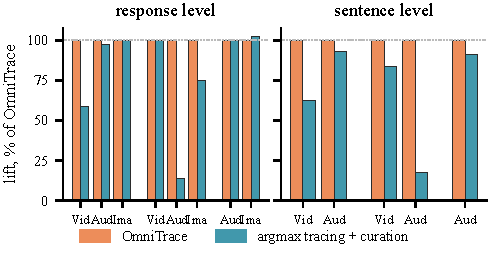
\includegraphics[width=\columnwidth]{media/figure/fig_transfer.pdf}
\caption{Lift of argmax tracing with curation as a share of OmniTrace's lift. In each panel the groups of bars are, from left to right, Qwen2.5-Omni-7B, on which the variant was developed, MiniCPM-o~4.5, and Qwen3-Omni-30B.}
\label{fig:transfer}
\end{figure}

\Cref{tab:models} compares OmniTrace with variants that change one design choice, and \Cref{fig:transfer} shows the comparison with hard tracing.
On Qwen2.5-Omni, argmax tracing with curation is level with OmniTrace on audio and image--text input and behind on video.
On MiniCPM-o~4.5 it loses most of its effect on audio, is behind on image--text input, and on video its top units are worse to keep than random ones.
On Qwen3-Omni-30B it is level with OmniTrace in lift on audio and image--text input, slightly ahead in keep gain, and behind at sentence level on audio; on video it keeps 60\% of the lift, as on Qwen2.5-Omni.
Using the last layer alone is reliably worse on audio for all three models, and on Qwen3-Omni it loses more than half of the lift in every modality.

The last rows hide the units that annotators marked.
On Qwen2.5-Omni, the units OmniTrace selects have a larger lift than the human-marked ones.
On Qwen3-Omni-30B the same holds for image--text input (0.316 against 0.267), and on video the two are close (0.033 against 0.027).
On MiniCPM-o~4.5 the order is reversed, most clearly on image--text input: there OmniTrace finds units that matter, but not the ones that matter most.

\subsection{Unit Size}
\label{appendix:size}

\begin{table}[t]
\centering
\tablesize
\setlength{\tabcolsep}{3.5pt}
% source: analysis/out/qwen2.5-omni-7b/unit_size.md (A)
\begin{tabular}{lccc}
\toprule
\textbf{Ranking} & $\rho$(score, size) & Top-1 size & Image share\\
\midrule
OmniTrace (sum) & $+$0.51 & 1.94 & 0.59\\
Per-token mean & $-$0.60 & 0.44 & 0.11\\
Leave-one-out & $+$0.09 & 1.62 & 0.48\\
ContextCite & $+$0.14 & 1.65 & 0.52\\
OmniTrace-trained & $+$0.08 & 1.71 & 0.52\\
Human evidence & $+$0.25 & 1.85 & 0.67\\
\bottomrule
\end{tabular}
\caption{Unit size on image--text input (Qwen2.5-Omni-7B). $\rho$: rank correlation between a quote's score and its token count, per question. Top-1 size: tokens of the top quote over the mean quote size. Image share: share of images among the top-ranked quotes.}
\label{tab:size}
\end{table}

\Cref{tab:size} gives the numbers behind \Cref{sec:size}. The per-token mean ranks short passages first and rarely an image. On MiniCPM-o~4.5 the mean is better than the sum at sentence level (\Cref{tab:models}), so the best correction for size depends on the model.

\subsection{Unit Granularity}
\label{appendix:granularity}

The score of a merged unit is the sum of its parts, but a selected set can still change with the unit length.
We merge one-second units into two- and four-second units and select the top 20\% of the duration again.
On video the selected time overlaps the one-second selection with IoU 0.60 and 0.50, where random rankings give 0.15; on audio the values are 0.53 and 0.42.
The selection is far from arbitrary but not invariant, so the unit length should be fixed and reported.

\subsection{Attribution Strength}
\label{appendix:flagging}

At sentence level, the attention mass a sentence places on the sources correlates with how much the sentence depends on them (rank correlation 0.60 on audio and image--text input, 0.26 on video, Qwen2.5-Omni).
At response level, a low share of mass on the audio flags wrong answers on Qwen2.5-Omni (AUROC 0.74), but not in the other modalities and not on MiniCPM-o~4.5.
Attribution strength thus indicates whether a sentence draws on the sources; it is not a general detector of wrong answers.

\section{Answer Accuracy of Long Answers}
\label{appendix:judge}

MMDocRAG answers are free text, so we grade them with an LLM judge (\texttt{claude-opus-5-5}).
The judge sees the question, the short and long reference answers, and the model's response, and returns \emph{correct} (all facts the reference needs), \emph{partial} (some facts right, at least one missing or wrong), or \emph{incorrect}. It does not see the quotes or images.
For Qwen2.5-Omni-7B, 374 of the 400 responses received a verdict: 23.8\% correct, 43.0\% partial, 33.2\% incorrect.
For MiniCPM-o~4.5 (400 verdicts): 50.5\% correct and 35.3\% partial.
For Qwen3-Omni-30B (400 verdicts): 54.0\% correct and 32.8\% partial.
The accuracy is used only to describe the models and to select correctly answered questions in \Cref{sec:agreement}.

\section{Data and Code}
We will release the code of OmniTrace, the causal tests, and the baselines, together with the question lists and the model responses used in this paper. The datasets keep the licenses of their creators.
